% ============================================================
% fig_loadings_matrix.tex
% Requer no preâmbulo:
%   \usepackage{tikz}
%   \usepackage{xcolor}
% ============================================================

\begin{figure}[htbp]
\centering
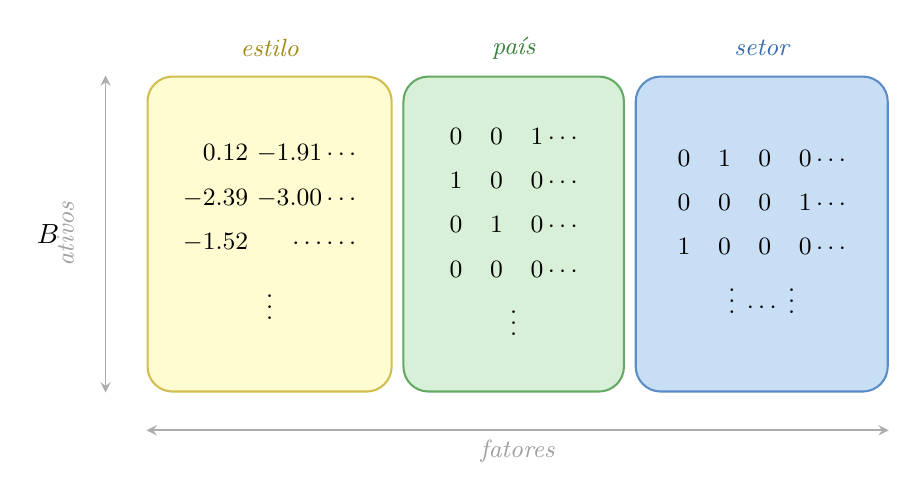
\begin{tikzpicture}[font=\small]

\definecolor{StyleFill}{RGB}{255,252,210}
\definecolor{StyleBorder}{RGB}{210,190,80}
\definecolor{StyleText}{RGB}{160,138,20}
\definecolor{CountryFill}{RGB}{215,240,215}
\definecolor{CountryBorder}{RGB}{100,170,100}
\definecolor{CountryText}{RGB}{60,130,60}
\definecolor{SectorFill}{RGB}{200,222,245}
\definecolor{SectorBorder}{RGB}{90,140,200}
\definecolor{SectorText}{RGB}{55,105,175}

% ── Bloco Estilo (x=0, w=3.1cm) ─────────────────────────────
\node[
    draw=StyleBorder, fill=StyleFill,
    rounded corners=9pt, line width=0.75pt,
    minimum width=3.1cm, minimum height=4.0cm,
    anchor=north west
] (style) at (0,0) {%
    $\begin{array}{r@{~}r@{~}l}
         0.12 & -1.91 & \!\cdots \\[5pt]
        -2.39 & -3.00 & \!\cdots \\[5pt]
        -1.52 & \cdots & \!\cdots \\[7pt]
        \multicolumn{3}{c}{\vdots}
    \end{array}$
};

% ── Bloco País (x=3.25cm, w=2.8cm) ──────────────────────────
\node[
    draw=CountryBorder, fill=CountryFill,
    rounded corners=9pt, line width=0.75pt,
    minimum width=2.8cm, minimum height=4.0cm,
    anchor=north west
] (country) at (3.25cm, 0) {%
    $\begin{array}{ccc@{~}l}
        0 & 0 & 1 & \!\cdots \\[5pt]
        1 & 0 & 0 & \!\cdots \\[5pt]
        0 & 1 & 0 & \!\cdots \\[5pt]
        0 & 0 & 0 & \!\cdots \\[3pt]
        \multicolumn{4}{c}{\vdots}
    \end{array}$
};

% ── Bloco Setor (x=6.2cm, w=3.1cm) ──────────────────────────
\node[
    draw=SectorBorder, fill=SectorFill,
    rounded corners=9pt, line width=0.75pt,
    minimum width=3.2cm, minimum height=4.0cm,
    anchor=north west
] (sector) at (6.2cm, 0) {%
    $\begin{array}{cccc@{~}l}
        0 & 1 & 0 & 0 & \!\cdots \\[5pt]
        0 & 0 & 0 & 1 & \!\cdots \\[5pt]
        1 & 0 & 0 & 0 & \!\cdots \\[3pt]
        \multicolumn{5}{c}{\vdots \;\cdots\; \vdots}
    \end{array}$
};

% ── Cabeçalhos em itálico colorido acima de cada bloco ──────
\node[StyleText,   font=\small\itshape] at ([yshift=0.35cm]style.north)   {estilo};
\node[CountryText, font=\small\itshape] at ([yshift=0.35cm]country.north) {pa\'{i}s};
\node[SectorText,  font=\small\itshape] at ([yshift=0.35cm]sector.north)  {setor};

% ── Seta horizontal "fatores" ────────────────────────────────
\draw[<->, >=stealth, line width=0.65pt, gray!65]
    ([yshift=-0.48cm]style.south west)
    -- node[below, font=\small\itshape, gray!75]{fatores}
    ([yshift=-0.48cm]sector.south east);

% ── Seta vertical + label "B  ativos" ───────────────────────
\draw[<->, >=stealth, line width=0.65pt, gray!65]
    ([xshift=-0.52cm]style.north west)
    --
    ([xshift=-0.52cm]style.south west);

% "ativos" rotacionado ao lado da seta
\node[font=\small\itshape, gray!75, rotate=90, anchor=south]
    at ([xshift=-0.80cm]style.west) {ativos};

% "B" à esquerda da seta
\node[font=\normalsize] at ([xshift=-1.25cm]style.west) {$B$};

\end{tikzpicture}
\caption{Estrutura típica da matriz de exposições fatoriais $B$,
particionada em blocos de estilo, pa\'{i}s e setor. As exposições de
estilo são valores contínuos padronizados; as exposições de pa\'{i}s e
setor são binárias, assumindo valor~1 se o ativo pertence àquela
categoria e 0 caso contrário \parencite{paleologo2025}.}
\label{fig:loadings_matrix}
\end{figure}